\newpage
\ESKDchecker{Дерябина}
\ESKDthisStyle{formII}
\section{Технико-экономическое обоснование}
\setcounter{figure}{0}

\subsection{Обоснование необходимости проводимого исследования}

В настоящее время автоматизированные системы коммерческого учета энергоресурсов(АСКУЭ) широко применяются на предприятиях. Это простой и эффективный способ контроля потребляемых предприятием ресурсов ресурсов. В настоящее время проводятся работы по реализации АСКУЭ, предназначенных для городских электросетей.

Изучая вопрос информационной безопасности таких систем, стало ясно
что существующие решения не подходят для использования, так как масштабы систем на предприятиях меньше и нет необходимости защищать систему от НСД, так как она находится в охраняемой зоне.

Цель данной работы — создать безопасный протокол взаимодействия устройства сбора и передачи данных (УСПД) с сервером сбора данных(ССД). На данном участке существующие протоколы плохо применимы ввиду больших расстояний и отсутствия защитных механизмов.

Для решения данной проблемы принято решение разработать новый протокол взаимодействия УСПД с ССД.

\subsection{Планирование комплекса работ по разработке программного обеспечения}

При выполнении дипломной работы было задействовано два человека:

\begin{itemize}
 \item руководитель;
 \item разработчик.
\end{itemize}

Руководитель выполняет контроль выполнения различных этапов работ, согласованность этапов выполнения работ между собой, корректирует действия разработчика, дает рекомендации по выполнению тех или иных работ. Разработчик реализует тот объем работ, который установлен руководителем в соответствие с техническим заданием.

Месячный оклад техника в ТУСУР составляет 3164 рубля, с учетом 20 рабочих дней в месяце, и 8 часового рабочего дня, стоимость одного часа работ равна 19,77 рублей. Месячный оклад руководителя к.н., доцента в университете равен 14 700 рублей\cite{money}, с учетом 24 рабочих дней, и 6 часового рабочего дня, стоимость одного часа работ равна 102,08 рубля.

График выполнения работ приведен в таблице 8.1.

Зная длительность цикла каждого этапа и возможность их параллельно-последовательного выполнения, можно рассчитать срок завершения планируемых работ и составить ленточный и сетевой графики плана их выполнения. Поскольку работа не требует большого состава исполнителей, то ограничимся ленточным графиком планирования, представленным в приложении \ref{app:lent_graf}.

 \includepdf[pages=3-7,fitpaper,
 addtotoc={4,subsection,2,Определение сметной стоимости проекта,eco3},
 ]{eco}
 
 \includepdf[pages=7-9,fitpaper,
 addtotoc={8,subsection,2,Экономический эффект,eco4}
 ]{eco}